Marcelo prepara brochetas como la siguiente con palitos y trozos de salchichas:

\begin{minipage}{0.4\linewidth}
    \begin{figure}[H]
        \centering
        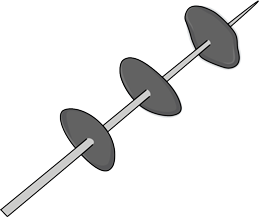
\includegraphics[width=0.9\linewidth]{../images/8cc56669378bdf27d863fffcaffb0080db06805e}
        \caption{Brocheta demostrativa}
        \label{fig:8cc56669378bdf27d863fffcaffb0080db06805e}
    \end{figure}
\end{minipage}\hfill
\begin{minipage}{0.6\linewidth}
    Para calcular cuántos palitos y cuántos trozos de salchicha necesitará, Marcelo elabora la siguiente tabla:

    \begin{table}[H]
        \centering
        \caption{}
        \label{tab:estampillas}
        \begin{tabular}{c|c|c|c|c|c|c}
            Cantidad de palitos             & 1 & 2 & 3 & 4  & \dots & 20 \\ \hline
            Cantidad de trozos de salchicha & 3 & 6 & 9 & 12 & \dots &    \\
        \end{tabular}
    \end{table}


    Si Marcelo cuenta la cantidad de trozos de salchicha que necesita para preparar
    20 palitos y luego suma todos los trozos que figuran en su tabla,
    \textbf{¿cuántos trozos obtendrá?}\\
\end{minipage}

\begin{solutionbox}{4cm}
    Ya que la regla de recurrencia es:
    \[a_n=3(n-1)+3\]
    entonces,
    \[a_{20}=3(20-1)+3=57+3=60\]
    y,
    \[s_{20}=\dfrac{20(a_0+a_{20})}{2}=\dfrac{20(3+60)}{2}=630 \text{ trozos.}\]
\end{solutionbox}
